%; whizzy paragraph -pdf xpdf -latex ./whizzypdfptex.sh
%; whizzy-paragraph "^\\\\begin{frame}"
% latex beamer presentation.
% platex, latex-beamer $B$G%3%s%Q%$%k$9$k$3$H$rA[Dj!#(B 

%     Tokyo Debian Meeting resources
%     Copyright (C) 2008 Junichi Uekawa

%     This program is free software; you can redistribute it and/or modify
%     it under the terms of the GNU General Public License as published by
%     the Free Software Foundation; either version 2 of the License, or
%     (at your option) any later version.

%     This program is distributed in the hope that it will be useful,
%     but WITHOUT ANY WARRANTY; without even the implied warranty of
%     MERCHANTABILITY or FITNESS FOR A PARTICULAR PURPOSE.  See the
%     GNU General Public License for more details.

%     You should have received a copy of the GNU General Public License
%     along with this program; if not, write to the Free Software
%     Foundation, Inc., 51 Franklin St, Fifth Floor, Boston, MA  02110-1301 USA

\documentclass[cjk,dvipdfm,12pt]{beamer}
\usetheme{Tokyo}
\usepackage{monthlypresentation}

%  preview (shell-command (concat "evince " (replace-regexp-in-string "tex$" "pdf"(buffer-file-name)) "&"))
%  presentation (shell-command (concat "xpdf -fullscreen " (replace-regexp-in-string "tex$" "pdf"(buffer-file-name)) "&"))
%  presentation (shell-command (concat "evince " (replace-regexp-in-string "tex$" "pdf"(buffer-file-name)) "&"))

%http://www.naney.org/diki/dk/hyperref.html
%$BF|K\8l(BEUC$B7O4D6-$N;~(B
\AtBeginDvi{\special{pdf:tounicode EUC-UCS2}}
%$B%7%U%H(BJIS$B7O4D6-$N;~(B
%\AtBeginDvi{\special{pdf:tounicode 90ms-RKSJ-UCS2}}

\title{$BEl5~%(%j%"(B Debian $BJY6/2q(B}
\subtitle{$B;qNA(B}
\author{$B>e@n(B $B=c0l(B dancer@debian.or.jp\\IRC nick: dancerj}
\date{2008$BG/(B12$B7n(B20$BF|(B}
\logo{
\includegraphics[width=8cm]{image200607/openlogo-light.eps}}

\begin{document}

\frame{\titlepage{}}

\emtext{$B@_1D=`Hw$K$46(NO$/$@$5$$(B}

\section{}
\begin{frame}
 \frametitle{Agenda}
\begin{minipage}[t]{0.45\hsize}
  \begin{itemize}
  \item $BCm0U;v9`(B
	\begin{itemize}
	 \item \underline{$B0{?)6X;_(B}
	 \item $B@/<#(B/$B=!65(B/$B1DMx3hF06X;_(B
	 \item ustream $B$K$F;n83%9%H%j!<%_%s%0Cf(B
	\end{itemize}
  \item $B:G6a$N(BDebian$B4XO"$N%$%Y%s%H(B
	\begin{itemize}
	 \item $BA02s$NJY6/2q(B
	\end{itemize}
 \end{itemize}
\end{minipage} 
\begin{minipage}[t]{0.45\hsize}
 \begin{itemize}
  \item Debian$B$N(B2008$BG/$r$U$j$+$($j!"(B2009$BG/$rM=A[$9$k(B
  \item $B%i%$%H%K%s%0%H!<%/(B
 \end{itemize}
\end{minipage}
\end{frame}

\section{$B:G6a(B}

\begin{frame}
 \frametitle{11$B7n(B}
\begin{minipage}[t]{0.45\hsize}
  \begin{itemize}
  \item $BCm0U;v9`(B
	\begin{itemize}
	 \item $B0{?)6X;_(B
	 \item $B@/<#(B/$B=!65(B/$B1DMx3hF06X;_(B
	 \item ustream $B$K$F;n83%9%H%j!<%_%s%0Cf(B
	\end{itemize}
  \item $B:G6a$N(BDebian$B4XO"$N%$%Y%s%H(B
	\begin{itemize}
	 \item $BA02s$NJY6/2q!"(BDebconf
	\end{itemize}
 \end{itemize}
\end{minipage} 
\begin{minipage}[t]{0.45\hsize}
 \begin{itemize}
  \item $B!V$=$N>l$GJY6/2q;qNA$r:n@.$7$A$c$(!W(B Debian $B$r;H$C$?(B LaTeX $B869F:n@.9g=I(B
 \end{itemize}
\end{minipage}
\end{frame}


\section{DWN quiz}
\begin{frame}{Debian $B>o<1%/%$%:(B}

Debian $B$N>o<1!"$b$A$m$sCN$C$F$^$9$h$M(B?
$BCN$i$J$$$J$s$FCQ$:$+$7$/$F!"CN$i$J$$$H$O8@$($J$$$"$s$J$3$H$d$3$s$J$3$H!"(B
$B$_$s$J$G3NG'$7$F$_$^$7$g$&!#(B

$B:#2s$N=PBjHO0O$O(B\url{debian-devel-announce@lists.deban.org} $B$KEj9F$5$l$?(B
$BFbMF$H(BDebian Project News$B$+$i$G$9!#(B

\end{frame}

\subsection{$BLdBj(B}

% TODO: fill here.

\section{$B:G6a$N(BDebian$B4XO"$N%$%Y%s%H(B}


\section{$B;vA02]Bj>R2p(B}
\emtext{$B;vA02]Bj$N>R2p(B}
% pre work home work

\begin{frame}{$B;vA02]Bj(B}

$B:#2s$N;vA02]Bj$O(B
$BA02s$N1i=,$rF'$^$($F(B \LaTeX{}$B$G:n@.$7$F$$$?$@$-$^$7$?!#(B
$B%H%T%C%/$O0J2<$NFs$D$N$&$A0l$D$rA*Br$9$k$3$H$K$J$C$F$$$^$7$?!#(B

\begin{enumerate}
 \item Debian$BJY6/2q$G:#G/$d$C$?$3$H!"MhG/$7$?$$$3$H(B
 \item \LaTeX{}+Git$B$N;vA02]Bj$,$G$-$J$+$C$?!"$3$s$J%O%^$jJ}$7$^$7$?BN835-(B
\end{enumerate}

\end{frame}

% (query-replace "\\subsection" "\\end{frame}\\begin{frame}")
% (query-replace "\\subsubsection" "\\textbf")

\emtext{2008$BG/7W2h(B}

\begin{frame}{2008$BG/7W2h(B}

{\scriptsize
\begin{enumerate}
 \item $B?7G/2q!V5$9g$rF~$l$k!W(B
 \item Open Source Conference Tokyo (3/1)
 \item $B%G!<%?$@$1$N%Q%C%1!<%8$r:n@.$7$F$_$k!"(B
       $B%i%$%;%s%9$N9M$(J}(B (David Smith)
 \item $B%P%$%J%j0l$D$N%Q%C%1!<%8$r:n@.$7$F$_$k(B ($B5HED(B@$BHD66(B)\\
       $B%P!<%8%g%s4IM}%D!<%k$r;H$$(BDebian$B%Q%C%1!<%8$r4IM}$9$k(B(git)\\
       $B%"%C%W%9%H%j!<%`$N07$$(B(svn/git/cvs)($B4d>>(B $B?.MN$5$s(B)
 \item $B%P%$%J%j$NJ,$1$?%Q%C%1!<%8$N:n@.!#(B($BA0ED$5$s(B)\\
       $B%P%$%J%j$NJ,$1J}$N9M$(J}!"%"%C%W%0%l!<%I$J$I$N1?MQ$H$+!#(B
 \item $B%Q%C%1!<%8:n@.(B(dpatch/debhelper$B$G:n@.$9$k%Q%C%1!<%8(B)($B>.NS576)$5$s(B)\\
       man $B$N=q$-J}(B(roff or docbook)($B$G$s$5$s(B)\\
       Open Source Conference Hokkaido
 \item $B%Q%C%1!<%8:n@.(B(kernel patch$B!"(Bkernel module)
       $B!"(BDebconf$BH/I=N}=,(B
 \item Debconf $B%"%k%<%s%A%s!"(BDebian$B29@t(B

 \item Open Source Conference Tokyo/Fall$B!"(B
       $B%G!<%b%s7O$N%Q%C%1!<%8$N:n@.!"(B\LaTeX{}$B!"(B emacs-lisp$B!"%U%)%s%H%Q%C%1!<%8(B
 \item $B%Q%C%1!<%8$N(B cross-compile $B$NJ}K!!"(Bamd64 $B>e$G(B i386 $B$N%Q%C%1!<%8$H(B
       $B$+!"(BOSC-Fall$BJs9p2q!"(BDebconf$BJs9p2q(B
 \item $B9q:]2=(B po-debconf / po$B2=(B / DDTP
 \item $BK:G/2q(B
\end{enumerate}
}
\end{frame}

\emtext{2008$BG/$N?6$jJV$j(B}

\section{}
\begin{frame}{$BEl5~%(%j%"(BDebian$BJY6/2q$N;22C<T$N?d0\(B}
 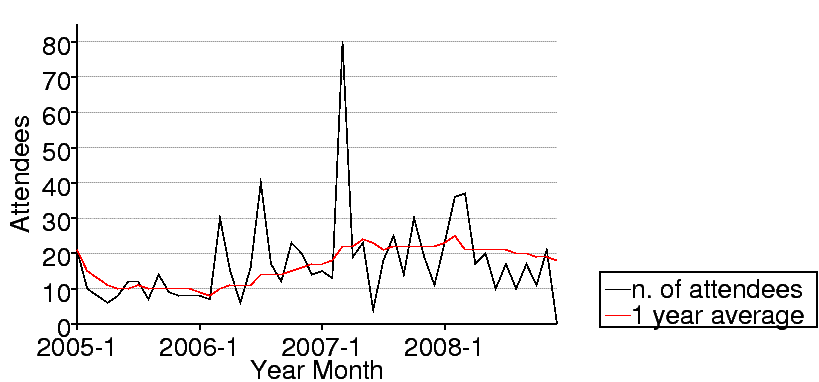
\includegraphics[width=1\hsize]{image200812/serialized.png}
\end{frame}

\begin{frame}{$B;vA02]Bj!&;v8e2]Bj$N?d0\(B}
 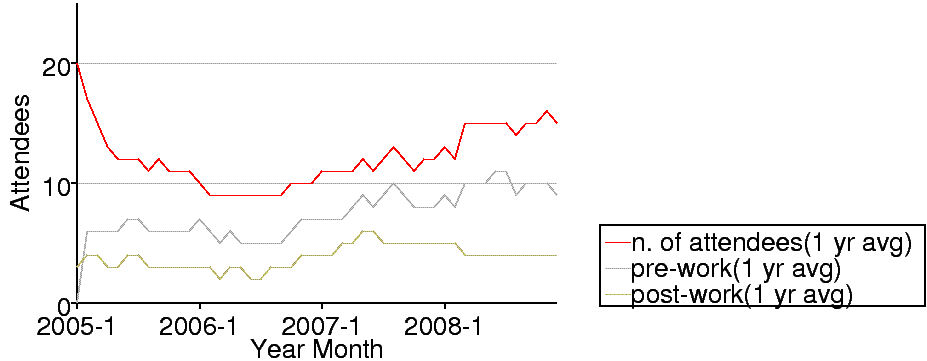
\includegraphics[width=1\hsize]{image200812/memberanalysis/attend.png}
\end{frame}

\begin{frame}{$B4X@>(BDebian$BJY6/2q$N;22C<T$N?d0\(B}
 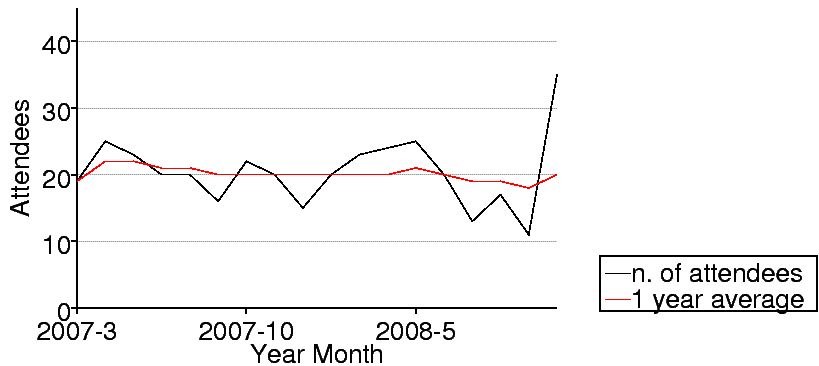
\includegraphics[width=1\hsize]{image200812/kansai.png}
\end{frame}

\emtext{2009$BG/$r7W2h$9$k(B}


\emtext{LT}

\emtext{sqlite3$B$r$D$+$C$F$_$?(B}
\section{sqlite3}
\begin{frame}{$B$O$8$a$K(B: sqlite3 $B$H$O(B?}

 $B$*<j7Z$J(BSQL$B%G!<%?%Y!<%9(B

 \fbox{\includegraphics[width=1\hsize]{image200812/sqlite.eps}}
\end{frame}

\begin{frame}[containsverbatim]{$B4JC1(B:$B%G!<%?%Y!<%9$N:n@.(B}

$B%G!<%?%Y!<%9$r:n@.$7$F$_$k(B!

\begin{commandline}
$ sqlite3 debmtg.db
sqlite> 
\end{commandline}

\end{frame}


\begin{frame}[containsverbatim]{$BFH<+$@$1$I4JC1$J%$%s%?%U%'!<%9(B}
\begin{commandline}
$ sqlite3 /tmp/a.db 
SQLite version 3.5.9
Enter ".help" for instructions
sqlite> create table unko(test text, count number); 
sqlite> .tables
unko
sqlite> .dump unko
BEGIN TRANSACTION;
CREATE TABLE unko(test text, count number);
COMMIT;
\end{commandline}
\end{frame}

\begin{frame}[containsverbatim]{$B8@8l%P%$%s%G%#%s%0(B}
\begin{commandline}
$ apt-cache search sqlite3 [$BH4?h(B]
cl-sql-sqlite3 - CLSQL database backend, SQLite3
libdbd-sqlite3 - SQLite3 database driver for libdbi
libdbd-sqlite3-perl - Perl DBI driver with a self-contained RDBMS
libdbd-sqlite3-ruby - Ruby/DBI driver for SQLite3
libdbd-sqlite3-ruby1.8 - Ruby/DBI SQLite driver for Ruby 1.8
libghc6-hdbc-sqlite3-dev - Sqlite v3 HDBC (Haskell Database Connectivity) Driver for GHC
libghc6-hsql-sqlite3-dev - SQLite driver of the HSQL library for GHC6
liblua5.1-sql-sqlite3-2 - luasql library for the lua language version 5.1
libsoci-sqlite3-gcc - C++ Database Access Library (SQLite3 backend)
libsqlite3-0 - SQLite 3 shared library
libsqlite3-gst - SQLite bindings for GNU Smalltalk
libsqlite3-ocaml - Embeddable SQL Database for OCaml Programs
libsqlite3-ocaml-dev - Embeddable SQL Database for OCaml Programs
libsqlite3-ruby - SQLite3 interface for Ruby
libsqlite3-tcl - SQLite 3 Tcl bindings
slang-sqlite - S-Lang bindings to the sqlite3 database library
\end{commandline} 
\end{frame}

\begin{frame}[containsverbatim]{python $B$NNc(B}
\begin{commandline}
from pysqlite2 import dbapi2
import csv

con = dbapi2.connect('debmtg.db')
cur = con.cursor()

cur.execute('create table test(name text, score number)')

for rows in csv.reader(file('test.csv')):
    cur.execute('insert into test(name, score) values(?,?)', 
                    (rows[0].decode('utf-8'),int(rows[1])))

con.commit()
con.close()

\end{commandline}
\end{frame}


\begin{frame}[containsverbatim]{python $B$NNc(B}
\begin{commandline}
from pysqlite2 import dbapi2
import csv
\end{commandline}

pysqlite2 $B$r%$%s%]!<%H$7$^$9!#(B

\end{frame}


\begin{frame}[containsverbatim]{python $B$NNc(B}
\begin{commandline}
con = dbapi2.connect('debmtg.db')
cur = con.cursor()
\end{commandline}

$B%G!<%?%Y!<%9$K%3%M%/%7%g%s$r$O$j$^$9!#(B
$BDL>o$N(BDB$B$@$H(BDB$B%5!<%P$K@\B3$9$k$N$@$1$I!"(Bsqlite3 $B$G$O%G!<%?%Y!<%9%U%!%$%k$r(B
 open$B$9$k=hM}AjEv!#(B

cursor $B$H$$$&$N$r%*!<%W%s$7$^$9!#A`:n$9$k$?$a$N%O%s%I%k$_$?$$$J$b$N!#(B

\end{frame}

\begin{frame}[containsverbatim]{python $B$NNc(B}
\begin{commandline}
cur.execute('create table test(name text, score number)')

for rows in csv.reader(file('test.csv')):
    cur.execute('insert into test(name, score) values(?,?)', 
                    (rows[0].decode('utf-8'),int(rows[1])))

\end{commandline}

cursor $B$N(B execute $B%3%^%s%I$GE,Ev$K(B SQL $BJ8$r<B9T$7$^$9!#(B
? $B$G;XDj$7$?ItJ,$r%Q%i%a!<%?CV49$7$F$/$l$k$N$,%]%$%s%H!#(B

\end{frame}

\begin{frame}[containsverbatim]{python $B$NNc(B}
\begin{commandline}
con.commit()
con.close()
\end{commandline}
$B%G!<%?%Y!<%9$X$N=q$-9~$_%H%i%s%6%/%7%g%s$r%3%_%C%H$7$F%/%m!<%:$7$^$9!#(B
$B%3%_%C%H(B(end transaction)$B$7$J$$$HH?1G$5$l$^$;$s!#(B
\end{frame}

\begin{frame}{$BJY6/J}K!(B}
\begin{itemize}
 \item SQL$B4XO"$N=q@R$J$I(B(Oracle, PostgreSQL, MySQL$B4XO"$O=<<B(B)$B!"0lIt(BDDL$B$O(B
       $B0c$&$N$GCm0U!#(B
 \item SQLite $B$N%*%s%i%$%s%I%-%e%a%s%F!<%7%g%s$r;29M$K$7$J$,$i$,$`$P$k(B?
\end{itemize}
\end{frame}

\emtext{$B<!2s$NJY6/2q(B}
\begin{frame}{$B<!2s$NJY6/2q(B}
$B<!2s$O?7G/2q$G$9!#(B
\end{frame}

\begin{frame}{$B1c2q>l=j(B}
\begin{itemize}
 \item $B1c2q>l=j(B\\
       $BK\F|$N1c2q$O!V(BXXXX$B!W$G$9!#(B\\
       $B;22C<T$O%U%m%"$K=89g$7!"A40w$G0\F0$7$^$7$g$&!#(B
 \item $BJRIU$1(B\\
       $BIt20$rJRIU$1$k$N$K$46(NO$/$@$5$$!#(B
\end{itemize}
\end{frame}

\end{document}

;;; Local Variables: ***
;;; outline-regexp: "\\([ 	]*\\\\\\(documentstyle\\|documentclass\\|emtext\\|section\\|begin{frame}\\)\\*?[ 	]*[[{]\\|[]+\\)" ***
;;; End: ***
